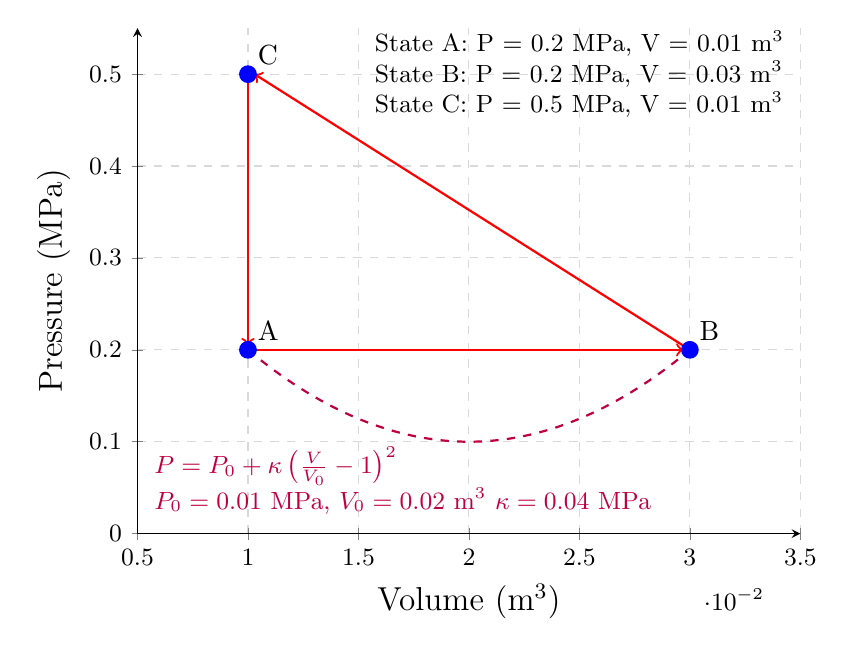
\begin{tikzpicture}
  \begin{axis}[
      xlabel={Volume (m$^3$)},
      ylabel={Pressure (MPa)},
      xmin=0.005, xmax=0.035,
      ymin=0.00, ymax=0.55,
      grid=major,
      grid style={dashed, gray!30},
      axis lines=left,
      width=10cm,
      height=8cm,
      tick label style={font=\small},
      label style={font=\large}
    ]

    % Define the three states
    \coordinate (A) at (0.01, 0.2);
    \coordinate (B) at (0.03, 0.2);
    \coordinate (C) at (0.01, 0.5);

    % Plot the points
    \addplot[only marks, mark=*, mark size=3pt, blue] coordinates {
      (0.01, 0.2)  % Point A
      (0.03, 0.2)  % Point B
      (0.01, 0.5)  % Point C
    };

    % Add labels for the points
    \node[above right] at (A) {A};
    \node[above right] at (B) {B};
    \node[above right] at (C) {C};

    % Draw arrows between states
    % Arrow A to B (horizontal, constant pressure)
    \draw[->, thick, red] (0.01, 0.2) -- (0.0297, 0.2);

    % Arrow B to C (vertical line, then to C)
    \draw[->, thick, red] (0.03, 0.2) -- (0.0103, 0.5);

    % Arrow C to A (vertical, constant volume)
    \draw[->, thick, red] (0.01, 0.5) -- (0.01, 0.205);

    % Add state information as text
    \node[align=left, font=\small] at (0.025, 0.5) {
      State A: P = 0.2 MPa, V = 0.01 m$^3$ \\
      State B: P = 0.2 MPa, V = 0.03 m$^3$ \\
      State C: P = 0.5 MPa, V = 0.01 m$^3$
    };

    % Plot the equation P = P_0 + κ(V/V_0 - 1)^2
    % where P_0 = 0.01 MPa, V_0 = 0.02 m^3, κ = 0.04 MPa
    \addplot[domain=0.01:0.03, samples=100, dashed, thick, purple]
    {0.1 + 0.4*((x/0.02) - 1)^2};

    % Add equation label
    \node[align=left, font=\small, purple] at (0.017, 0.058) {
      $P = P_0 + \kappa\left(\frac{V}{V_0} - 1\right)^2$ \\
      $P_0 = 0.01$ MPa, $V_0 = 0.02$ m$^3$ $\kappa = 0.04$ MPa
    };

  \end{axis}
\end{tikzpicture}
